% Created by tikzDevice version 0.12.6 on 2025-12-23 06:21:21
% !TEX encoding = UTF-8 Unicode
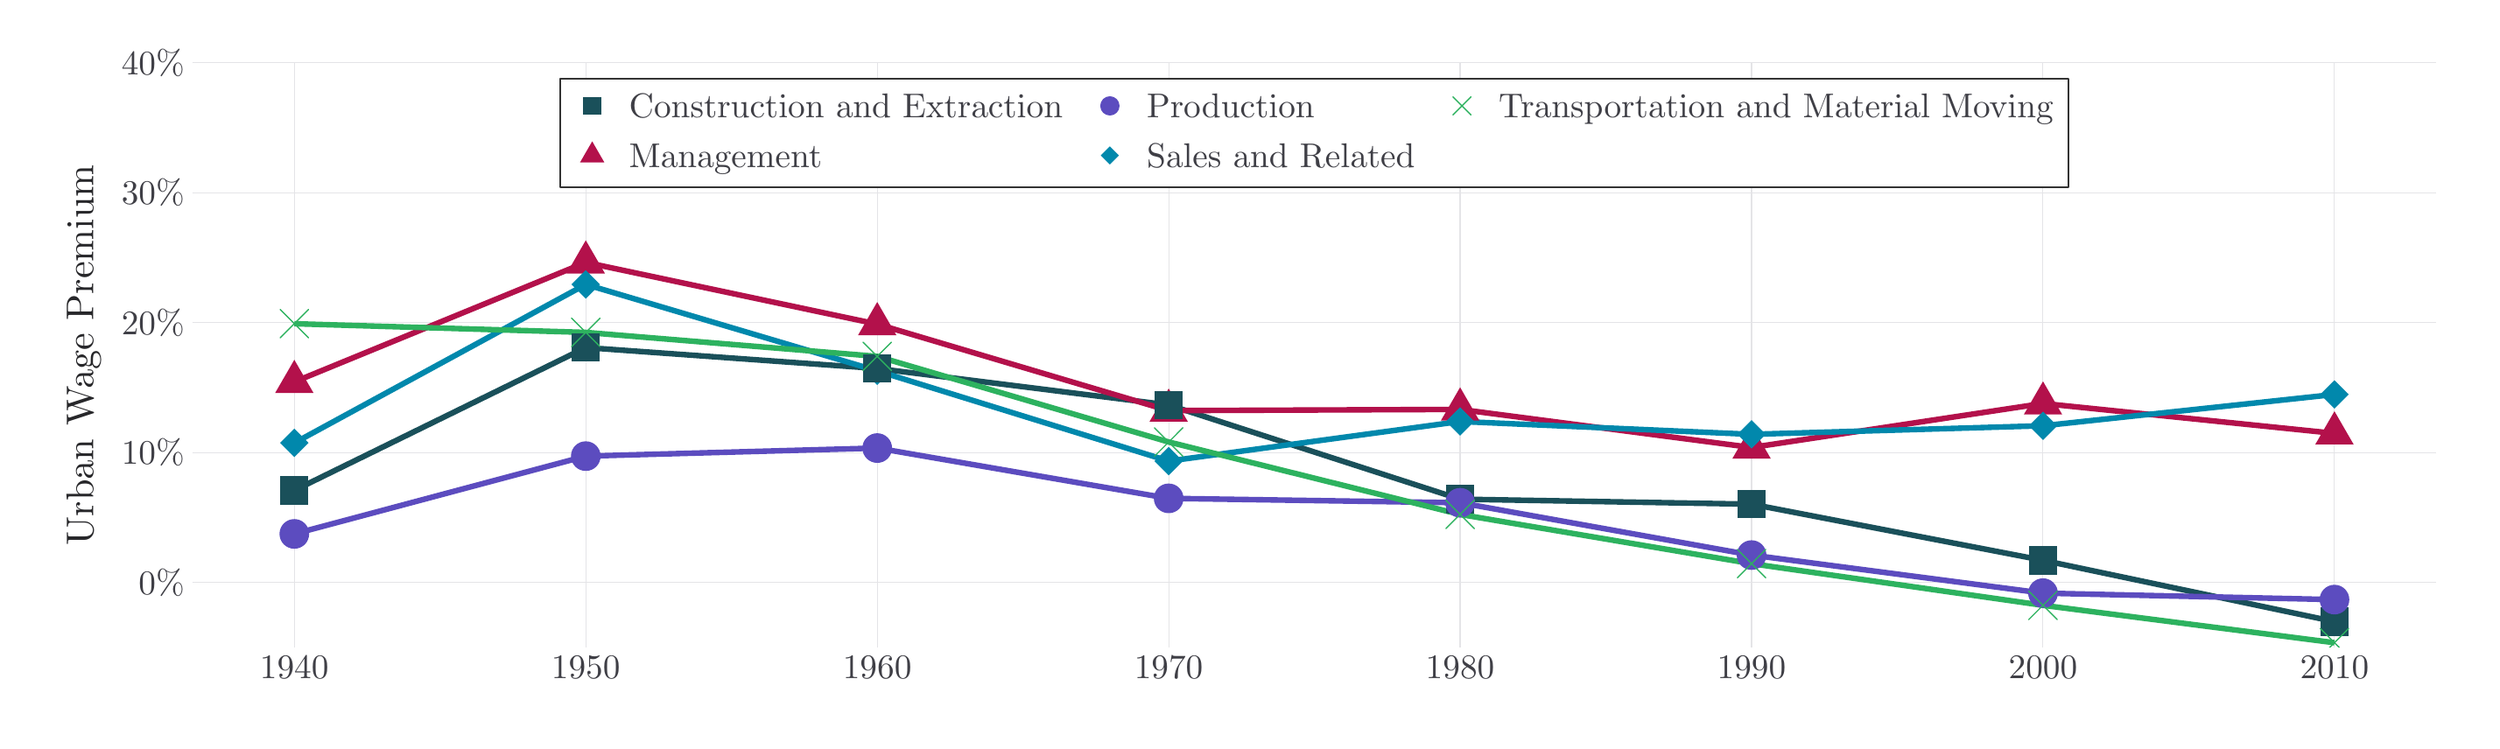
\begin{tikzpicture}[x=1pt,y=1pt]
\definecolor{fillColor}{RGB}{255,255,255}
\path[use as bounding box,fill=fillColor] (0,0) rectangle (1011.78,289.08);
\begin{scope}
\path[clip] (  0.00,  0.00) rectangle (1011.78,289.08);
\definecolor{drawColor}{RGB}{255,255,255}

\path[draw=drawColor,line width= 0.8pt,line join=round,line cap=round,fill=fillColor] (  0.00,  0.00) rectangle (1011.78,289.08);
\end{scope}
\begin{scope}
\path[clip] ( 69.39, 31.76) rectangle (995.78,273.08);
\definecolor{drawColor}{RGB}{255,255,255}
\definecolor{fillColor}{RGB}{255,255,255}

\path[draw=drawColor,line width= 0.8pt,line join=round,line cap=round,fill=fillColor] ( 69.39, 31.76) rectangle (995.78,273.08);
\definecolor{drawColor}{RGB}{228,228,231}

\path[draw=drawColor,line width= 0.4pt,line join=round] ( 69.39, 58.57) --
	(995.78, 58.57);

\path[draw=drawColor,line width= 0.4pt,line join=round] ( 69.39,112.20) --
	(995.78,112.20);

\path[draw=drawColor,line width= 0.4pt,line join=round] ( 69.39,165.83) --
	(995.78,165.83);

\path[draw=drawColor,line width= 0.4pt,line join=round] ( 69.39,219.45) --
	(995.78,219.45);

\path[draw=drawColor,line width= 0.4pt,line join=round] ( 69.39,273.08) --
	(995.78,273.08);

\path[draw=drawColor,line width= 0.4pt,line join=round] (111.50, 31.76) --
	(111.50,273.08);

\path[draw=drawColor,line width= 0.4pt,line join=round] (231.81, 31.76) --
	(231.81,273.08);

\path[draw=drawColor,line width= 0.4pt,line join=round] (352.12, 31.76) --
	(352.12,273.08);

\path[draw=drawColor,line width= 0.4pt,line join=round] (472.43, 31.76) --
	(472.43,273.08);

\path[draw=drawColor,line width= 0.4pt,line join=round] (592.74, 31.76) --
	(592.74,273.08);

\path[draw=drawColor,line width= 0.4pt,line join=round] (713.05, 31.76) --
	(713.05,273.08);

\path[draw=drawColor,line width= 0.4pt,line join=round] (833.36, 31.76) --
	(833.36,273.08);

\path[draw=drawColor,line width= 0.4pt,line join=round] (953.67, 31.76) --
	(953.67,273.08);
\definecolor{drawColor}{RGB}{26,80,90}

\path[draw=drawColor,line width= 2.3pt,line join=round] (111.50, 96.56) --
	(231.81,155.54) --
	(352.12,146.90) --
	(472.43,131.85) --
	(592.74, 92.93) --
	(713.05, 90.87) --
	(833.36, 67.69) --
	(953.67, 42.38);
\definecolor{drawColor}{RGB}{179,17,75}

\path[draw=drawColor,line width= 2.3pt,line join=round] (111.50,141.37) --
	(231.81,190.71) --
	(352.12,165.22) --
	(472.43,129.51) --
	(592.74,130.00) --
	(713.05,114.29) --
	(833.36,132.45) --
	(953.67,120.12);
\definecolor{drawColor}{RGB}{92,76,191}

\path[draw=drawColor,line width= 2.3pt,line join=round] (111.50, 78.59) --
	(231.81,110.71) --
	(352.12,114.04) --
	(472.43, 93.27) --
	(592.74, 91.45) --
	(713.05, 69.85) --
	(833.36, 54.13) --
	(953.67, 51.46);
\definecolor{drawColor}{RGB}{1,136,172}

\path[draw=drawColor,line width= 2.3pt,line join=round] (111.50,116.15) --
	(231.81,181.62) --
	(352.12,145.93) --
	(472.43,108.67) --
	(592.74,125.02) --
	(713.05,119.71) --
	(833.36,123.25) --
	(953.67,136.18);
\definecolor{drawColor}{RGB}{45,178,95}

\path[draw=drawColor,line width= 2.3pt,line join=round] (111.50,165.39) --
	(231.81,161.80) --
	(352.12,151.90) --
	(472.43,116.55) --
	(592.74, 86.64) --
	(713.05, 66.30) --
	(833.36, 49.10) --
	(953.67, 33.66);
\definecolor{fillColor}{RGB}{179,17,75}

\path[fill=fillColor] (111.50,150.50) --
	(119.41,136.80) --
	(103.59,136.80) --
	cycle;
\definecolor{fillColor}{RGB}{1,136,172}

\path[fill=fillColor] (105.63,116.15) --
	(111.50,122.02) --
	(117.37,116.15) --
	(111.50,110.28) --
	cycle;
\definecolor{fillColor}{RGB}{26,80,90}

\path[fill=fillColor] (105.63, 90.69) --
	(117.37, 90.69) --
	(117.37,102.43) --
	(105.63,102.43) --
	cycle;
\definecolor{drawColor}{RGB}{92,76,191}
\definecolor{fillColor}{RGB}{92,76,191}

\path[draw=drawColor,line width= 0.5pt,line join=round,line cap=round,fill=fillColor] (111.50, 78.59) circle (  5.87);
\definecolor{drawColor}{RGB}{45,178,95}

\path[draw=drawColor,line width= 0.5pt,line join=round,line cap=round] (105.63,159.52) -- (117.37,171.26);

\path[draw=drawColor,line width= 0.5pt,line join=round,line cap=round] (105.63,171.26) -- (117.37,159.52);
\definecolor{fillColor}{RGB}{179,17,75}

\path[fill=fillColor] (231.81,199.84) --
	(239.72,186.14) --
	(223.90,186.14) --
	cycle;
\definecolor{fillColor}{RGB}{1,136,172}

\path[fill=fillColor] (225.94,181.62) --
	(231.81,187.49) --
	(237.68,181.62) --
	(231.81,175.74) --
	cycle;
\definecolor{fillColor}{RGB}{26,80,90}

\path[fill=fillColor] (225.94,149.66) --
	(237.68,149.66) --
	(237.68,161.41) --
	(225.94,161.41) --
	cycle;
\definecolor{drawColor}{RGB}{92,76,191}
\definecolor{fillColor}{RGB}{92,76,191}

\path[draw=drawColor,line width= 0.5pt,line join=round,line cap=round,fill=fillColor] (231.81,110.71) circle (  5.87);
\definecolor{drawColor}{RGB}{45,178,95}

\path[draw=drawColor,line width= 0.5pt,line join=round,line cap=round] (225.94,155.93) -- (237.68,167.67);

\path[draw=drawColor,line width= 0.5pt,line join=round,line cap=round] (225.94,167.67) -- (237.68,155.93);
\definecolor{fillColor}{RGB}{179,17,75}

\path[fill=fillColor] (352.12,174.36) --
	(360.03,160.66) --
	(344.21,160.66) --
	cycle;
\definecolor{fillColor}{RGB}{1,136,172}

\path[fill=fillColor] (346.25,145.93) --
	(352.12,151.81) --
	(357.99,145.93) --
	(352.12,140.06) --
	cycle;
\definecolor{fillColor}{RGB}{26,80,90}

\path[fill=fillColor] (346.25,141.02) --
	(357.99,141.02) --
	(357.99,152.77) --
	(346.25,152.77) --
	cycle;
\definecolor{drawColor}{RGB}{92,76,191}
\definecolor{fillColor}{RGB}{92,76,191}

\path[draw=drawColor,line width= 0.5pt,line join=round,line cap=round,fill=fillColor] (352.12,114.04) circle (  5.87);
\definecolor{drawColor}{RGB}{45,178,95}

\path[draw=drawColor,line width= 0.5pt,line join=round,line cap=round] (346.25,146.03) -- (357.99,157.77);

\path[draw=drawColor,line width= 0.5pt,line join=round,line cap=round] (346.25,157.77) -- (357.99,146.03);
\definecolor{fillColor}{RGB}{179,17,75}

\path[fill=fillColor] (472.43,138.64) --
	(480.34,124.95) --
	(464.52,124.95) --
	cycle;
\definecolor{fillColor}{RGB}{1,136,172}

\path[fill=fillColor] (466.56,108.67) --
	(472.43,114.55) --
	(478.30,108.67) --
	(472.43,102.80) --
	cycle;
\definecolor{fillColor}{RGB}{26,80,90}

\path[fill=fillColor] (466.56,125.98) --
	(478.30,125.98) --
	(478.30,137.73) --
	(466.56,137.73) --
	cycle;
\definecolor{drawColor}{RGB}{92,76,191}
\definecolor{fillColor}{RGB}{92,76,191}

\path[draw=drawColor,line width= 0.5pt,line join=round,line cap=round,fill=fillColor] (472.43, 93.27) circle (  5.87);
\definecolor{drawColor}{RGB}{45,178,95}

\path[draw=drawColor,line width= 0.5pt,line join=round,line cap=round] (466.56,110.67) -- (478.30,122.42);

\path[draw=drawColor,line width= 0.5pt,line join=round,line cap=round] (466.56,122.42) -- (478.30,110.67);
\definecolor{fillColor}{RGB}{179,17,75}

\path[fill=fillColor] (592.74,139.13) --
	(600.65,125.43) --
	(584.83,125.43) --
	cycle;
\definecolor{fillColor}{RGB}{1,136,172}

\path[fill=fillColor] (586.87,125.02) --
	(592.74,130.89) --
	(598.61,125.02) --
	(592.74,119.15) --
	cycle;
\definecolor{fillColor}{RGB}{26,80,90}

\path[fill=fillColor] (586.87, 87.05) --
	(598.61, 87.05) --
	(598.61, 98.80) --
	(586.87, 98.80) --
	cycle;
\definecolor{drawColor}{RGB}{92,76,191}
\definecolor{fillColor}{RGB}{92,76,191}

\path[draw=drawColor,line width= 0.5pt,line join=round,line cap=round,fill=fillColor] (592.74, 91.45) circle (  5.87);
\definecolor{drawColor}{RGB}{45,178,95}

\path[draw=drawColor,line width= 0.5pt,line join=round,line cap=round] (586.87, 80.77) -- (598.61, 92.52);

\path[draw=drawColor,line width= 0.5pt,line join=round,line cap=round] (586.87, 92.52) -- (598.61, 80.77);
\definecolor{fillColor}{RGB}{179,17,75}

\path[fill=fillColor] (713.05,123.42) --
	(720.96,109.72) --
	(705.14,109.72) --
	cycle;
\definecolor{fillColor}{RGB}{1,136,172}

\path[fill=fillColor] (707.18,119.71) --
	(713.05,125.58) --
	(718.92,119.71) --
	(713.05,113.83) --
	cycle;
\definecolor{fillColor}{RGB}{26,80,90}

\path[fill=fillColor] (707.18, 85.00) --
	(718.92, 85.00) --
	(718.92, 96.74) --
	(707.18, 96.74) --
	cycle;
\definecolor{drawColor}{RGB}{92,76,191}
\definecolor{fillColor}{RGB}{92,76,191}

\path[draw=drawColor,line width= 0.5pt,line join=round,line cap=round,fill=fillColor] (713.05, 69.85) circle (  5.87);
\definecolor{drawColor}{RGB}{45,178,95}

\path[draw=drawColor,line width= 0.5pt,line join=round,line cap=round] (707.18, 60.43) -- (718.92, 72.17);

\path[draw=drawColor,line width= 0.5pt,line join=round,line cap=round] (707.18, 72.17) -- (718.92, 60.43);
\definecolor{fillColor}{RGB}{179,17,75}

\path[fill=fillColor] (833.36,141.59) --
	(841.27,127.89) --
	(825.45,127.89) --
	cycle;
\definecolor{fillColor}{RGB}{1,136,172}

\path[fill=fillColor] (827.49,123.25) --
	(833.36,129.12) --
	(839.23,123.25) --
	(833.36,117.38) --
	cycle;
\definecolor{fillColor}{RGB}{26,80,90}

\path[fill=fillColor] (827.49, 61.82) --
	(839.23, 61.82) --
	(839.23, 73.56) --
	(827.49, 73.56) --
	cycle;
\definecolor{drawColor}{RGB}{92,76,191}
\definecolor{fillColor}{RGB}{92,76,191}

\path[draw=drawColor,line width= 0.5pt,line join=round,line cap=round,fill=fillColor] (833.36, 54.13) circle (  5.87);
\definecolor{drawColor}{RGB}{45,178,95}

\path[draw=drawColor,line width= 0.5pt,line join=round,line cap=round] (827.49, 43.23) -- (839.23, 54.97);

\path[draw=drawColor,line width= 0.5pt,line join=round,line cap=round] (827.49, 54.97) -- (839.23, 43.23);
\definecolor{fillColor}{RGB}{179,17,75}

\path[fill=fillColor] (953.67,129.25) --
	(961.58,115.55) --
	(945.76,115.55) --
	cycle;
\definecolor{fillColor}{RGB}{1,136,172}

\path[fill=fillColor] (947.80,136.18) --
	(953.67,142.05) --
	(959.54,136.18) --
	(953.67,130.31) --
	cycle;
\definecolor{fillColor}{RGB}{26,80,90}

\path[fill=fillColor] (947.80, 36.51) --
	(959.54, 36.51) --
	(959.54, 48.25) --
	(947.80, 48.25) --
	cycle;
\definecolor{drawColor}{RGB}{92,76,191}
\definecolor{fillColor}{RGB}{92,76,191}

\path[draw=drawColor,line width= 0.5pt,line join=round,line cap=round,fill=fillColor] (953.67, 51.46) circle (  5.87);
\definecolor{drawColor}{RGB}{45,178,95}

\path[draw=drawColor,line width= 0.5pt,line join=round,line cap=round] (947.80, 27.79) -- (959.54, 39.54);

\path[draw=drawColor,line width= 0.5pt,line join=round,line cap=round] (947.80, 39.54) -- (959.54, 27.79);
\end{scope}
\begin{scope}
\path[clip] (  0.00,  0.00) rectangle (1011.78,289.08);
\definecolor{drawColor}{RGB}{63,63,70}

\node[text=drawColor,anchor=base east,inner sep=0pt, outer sep=0pt, scale=  1.42] at ( 66.19, 53.67) {0\%};

\node[text=drawColor,anchor=base east,inner sep=0pt, outer sep=0pt, scale=  1.42] at ( 66.19,107.30) {10\%};

\node[text=drawColor,anchor=base east,inner sep=0pt, outer sep=0pt, scale=  1.42] at ( 66.19,160.93) {20\%};

\node[text=drawColor,anchor=base east,inner sep=0pt, outer sep=0pt, scale=  1.42] at ( 66.19,214.56) {30\%};

\node[text=drawColor,anchor=base east,inner sep=0pt, outer sep=0pt, scale=  1.42] at ( 66.19,268.18) {40\%};
\end{scope}
\begin{scope}
\path[clip] (  0.00,  0.00) rectangle (1011.78,289.08);
\definecolor{drawColor}{RGB}{63,63,70}

\node[text=drawColor,anchor=base,inner sep=0pt, outer sep=0pt, scale=  1.42] at (111.50, 18.76) {1940};

\node[text=drawColor,anchor=base,inner sep=0pt, outer sep=0pt, scale=  1.42] at (231.81, 18.76) {1950};

\node[text=drawColor,anchor=base,inner sep=0pt, outer sep=0pt, scale=  1.42] at (352.12, 18.76) {1960};

\node[text=drawColor,anchor=base,inner sep=0pt, outer sep=0pt, scale=  1.42] at (472.43, 18.76) {1970};

\node[text=drawColor,anchor=base,inner sep=0pt, outer sep=0pt, scale=  1.42] at (592.74, 18.76) {1980};

\node[text=drawColor,anchor=base,inner sep=0pt, outer sep=0pt, scale=  1.42] at (713.05, 18.76) {1990};

\node[text=drawColor,anchor=base,inner sep=0pt, outer sep=0pt, scale=  1.42] at (833.36, 18.76) {2000};

\node[text=drawColor,anchor=base,inner sep=0pt, outer sep=0pt, scale=  1.42] at (953.67, 18.76) {2010};
\end{scope}
\begin{scope}
\path[clip] (  0.00,  0.00) rectangle (1011.78,289.08);
\definecolor{drawColor}{RGB}{39,39,42}

\node[text=drawColor,rotate= 90.00,anchor=base,inner sep=0pt, outer sep=0pt, scale=  1.60] at ( 28.57,152.42) {Urban Wage Premium};
\end{scope}
\begin{scope}
\path[clip] (  0.00,  0.00) rectangle (1011.78,289.08);
\definecolor{drawColor}{gray}{0.20}
\definecolor{fillColor}{RGB}{255,255,255}

\path[draw=drawColor,line width= 0.8pt,line join=round,line cap=round,fill=fillColor] (221.24,221.67) rectangle (843.94,266.58);
\end{scope}
\begin{scope}
\path[clip] (  0.00,  0.00) rectangle (1011.78,289.08);
\definecolor{drawColor}{RGB}{255,255,255}
\definecolor{fillColor}{RGB}{255,255,255}

\path[draw=drawColor,line width= 0.8pt,line join=round,line cap=round,fill=fillColor] (227.24,248.12) rectangle (241.69,262.58);

\path[] (228.68,255.35) -- (240.25,255.35);
\definecolor{fillColor}{RGB}{26,80,90}

\path[fill=fillColor] (230.73,251.62) --
	(238.19,251.62) --
	(238.19,259.08) --
	(230.73,259.08) --
	cycle;
\end{scope}
\begin{scope}
\path[clip] (  0.00,  0.00) rectangle (1011.78,289.08);
\definecolor{drawColor}{RGB}{255,255,255}
\definecolor{fillColor}{RGB}{255,255,255}

\path[draw=drawColor,line width= 0.8pt,line join=round,line cap=round,fill=fillColor] (227.24,227.67) rectangle (241.69,242.12);

\path[] (228.68,234.89) -- (240.25,234.89);
\definecolor{fillColor}{RGB}{179,17,75}

\path[fill=fillColor] (234.46,240.70) --
	(239.49,231.99) --
	(229.44,231.99) --
	cycle;
\end{scope}
\begin{scope}
\path[clip] (  0.00,  0.00) rectangle (1011.78,289.08);
\definecolor{drawColor}{RGB}{255,255,255}
\definecolor{fillColor}{RGB}{255,255,255}

\path[draw=drawColor,line width= 0.8pt,line join=round,line cap=round,fill=fillColor] (440.94,248.12) rectangle (455.39,262.58);

\path[] (442.38,255.35) -- (453.95,255.35);
\definecolor{drawColor}{RGB}{92,76,191}
\definecolor{fillColor}{RGB}{92,76,191}

\path[draw=drawColor,line width= 0.5pt,line join=round,line cap=round,fill=fillColor] (448.16,255.35) circle (  3.73);
\end{scope}
\begin{scope}
\path[clip] (  0.00,  0.00) rectangle (1011.78,289.08);
\definecolor{drawColor}{RGB}{255,255,255}
\definecolor{fillColor}{RGB}{255,255,255}

\path[draw=drawColor,line width= 0.8pt,line join=round,line cap=round,fill=fillColor] (440.94,227.67) rectangle (455.39,242.12);

\path[] (442.38,234.89) -- (453.95,234.89);
\definecolor{fillColor}{RGB}{1,136,172}

\path[fill=fillColor] (444.43,234.89) --
	(448.16,238.62) --
	(451.90,234.89) --
	(448.16,231.16) --
	cycle;
\end{scope}
\begin{scope}
\path[clip] (  0.00,  0.00) rectangle (1011.78,289.08);
\definecolor{drawColor}{RGB}{255,255,255}
\definecolor{fillColor}{RGB}{255,255,255}

\path[draw=drawColor,line width= 0.8pt,line join=round,line cap=round,fill=fillColor] (586.24,248.12) rectangle (600.69,262.58);

\path[] (587.69,255.35) -- (599.25,255.35);
\definecolor{drawColor}{RGB}{45,178,95}

\path[draw=drawColor,line width= 0.5pt,line join=round,line cap=round] (589.74,251.62) -- (597.20,259.08);

\path[draw=drawColor,line width= 0.5pt,line join=round,line cap=round] (589.74,259.08) -- (597.20,251.62);
\end{scope}
\begin{scope}
\path[clip] (  0.00,  0.00) rectangle (1011.78,289.08);
\definecolor{drawColor}{RGB}{63,63,70}

\node[text=drawColor,anchor=base west,inner sep=0pt, outer sep=0pt, scale=  1.42] at (249.69,250.45) {Construction and Extraction};
\end{scope}
\begin{scope}
\path[clip] (  0.00,  0.00) rectangle (1011.78,289.08);
\definecolor{drawColor}{RGB}{63,63,70}

\node[text=drawColor,anchor=base west,inner sep=0pt, outer sep=0pt, scale=  1.42] at (249.69,230.00) {Management};
\end{scope}
\begin{scope}
\path[clip] (  0.00,  0.00) rectangle (1011.78,289.08);
\definecolor{drawColor}{RGB}{63,63,70}

\node[text=drawColor,anchor=base west,inner sep=0pt, outer sep=0pt, scale=  1.42] at (463.39,250.45) {Production};
\end{scope}
\begin{scope}
\path[clip] (  0.00,  0.00) rectangle (1011.78,289.08);
\definecolor{drawColor}{RGB}{63,63,70}

\node[text=drawColor,anchor=base west,inner sep=0pt, outer sep=0pt, scale=  1.42] at (463.39,230.00) {Sales and Related};
\end{scope}
\begin{scope}
\path[clip] (  0.00,  0.00) rectangle (1011.78,289.08);
\definecolor{drawColor}{RGB}{63,63,70}

\node[text=drawColor,anchor=base west,inner sep=0pt, outer sep=0pt, scale=  1.42] at (608.69,250.45) {Transportation and Material Moving};
\end{scope}
\end{tikzpicture}
